\subsection{Model-view-controller (Jens Carl)}
We chose to develop our application from the Model-view-controller design pattern. For an overview of MVC and our class implementation see figure \ref{fig:MVC_CD}

The MVC design pattern is our team's most familiar design/architecture pattern to develop from. We've used it, and been taught it, in past projects in previous courses\footnote{DTU courses 02121 Intro to Software Tech, 02161 Software Engineering 1} to great success. The MVC pattern is simple to implement in group-work since work on independent parts can be split up. During development it helps keep up the workflow with either a top-down approach (starting from the controller and working downwards towards the elementary data model) or bottom-up (implementing the data model first and then using it in controller methods). For long term development, the MVC provide relatively good flexibility for changing plans (e.g. changing data structure) mid-term. The old model can be reused for a different purpose by re-routing in the controller, and previously made view classes (front-end) can remain mostly unchanged while the back-end is reworked.  
All in all, choosing MVC provides us with an experienced starting point and fits well into the scope of the project.

\begin{figure}[H]
\centering
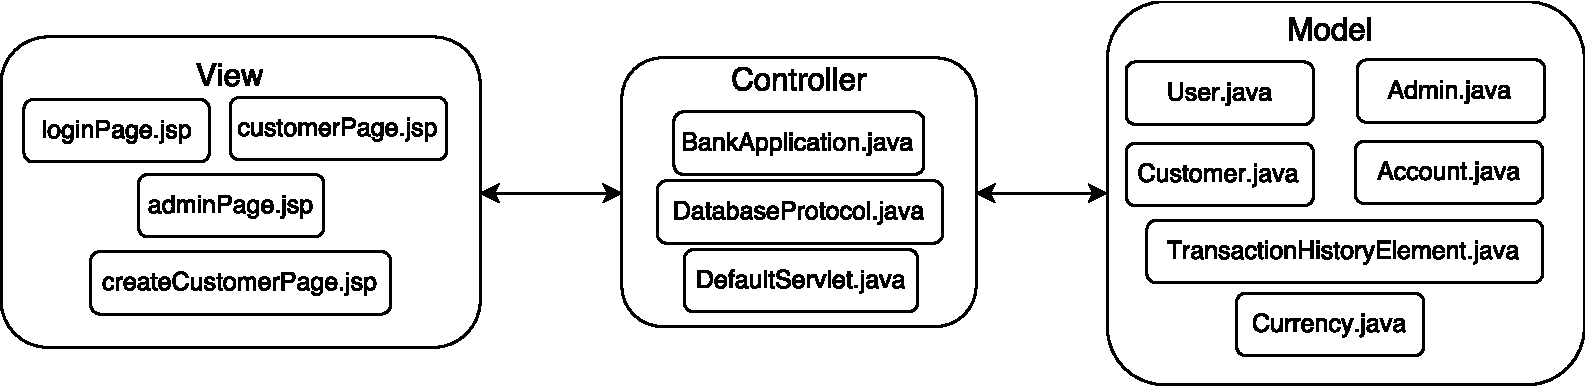
\includegraphics[width = 1.00\textwidth]{figures/class_diagram_abridged.pdf}
\caption{Diagram showcasing how we divided our classes into the three MVC components. The web layout files are in the View component. They register user input and send it to the Controller. The controller consist of Java classes governing the main logic in the application. Based on the signal from View, it tells the Model which changes in data that need to occur. Data in the Model can in turn provoke the Controller to make new changes, and in the end the Controller sends back to View what should be displayed to the user.}
\label{fig:MVC_CD}
\end{figure}